\section{Il contesto}
Una \textbf{time series}\footnote{Nel seguito verrà usato anche \textit{TS}} (serie temporale) è una serie di dati ordinati nel tempo. Tipicamente, i dati sono presi ad intervalli di tempo regolari. Alcuni esempi sono gli elettrocardiogrammi, l'andamento delle maree, i valori azionari.
\begin{figure}[H]
	\centering
	%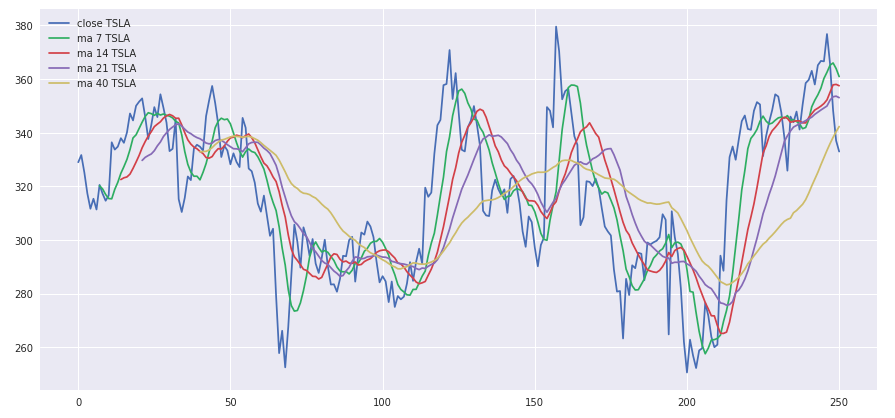
\includegraphics[width=\linewidth]{timeseries.png}
	\caption{Un'insieme di TS, ciascuna di colore diverso}
	\label{fig:timeseries}
\end{figure}
Le TS, quindi, sono molti simili a dei segnali, quindi analizzabili sia in dominio del tempo che in dominio della frequenza.\\
\\
L'\textbf{analisi di time series} si occupa di analizzare questi dati per estrarre informazioni statisticamente rilevanti per diversi scopi:
\begin{itemize}
	\item \textbf{Previsioni}, per prevedere andamento di alcuni eventi nel futuro, come le azioni in borsa, oscillazioni della terra, tramite un modello statistico;
	\item \textbf{Stime}, per approssimare l'informazione portata da segnali di vario genere;
	\item \textbf{Anomaly detection}, per identificare alcuni pattern ricorrenti sospetti.
\end{itemize}
Per portare a termine questi scopi, i principali task sulle TS sono:
\begin{itemize}
	\item \textbf{Classificazione}, che consiste nella costruzione di un modello che apprende dai dati (le TS) il modo in cui assegnare a ciascuna di loro una label. Il modello può essere basato su SVM, k-NN, reti neurali, regressione o alberi di decisione. L'apprendimento è di tipo supervisionato, quindi sono necessarie delle label assegnate ai dati di addestramento;
	\item \textbf{Clustering}, che consiste nel partizionare un insieme di TS a seconda della loro similarità. Bisogna dapprima scegliere una metrica di similarità (o distanza), come può essere la distanza Euclidea o la tecnica del DTW\footnote{Dynamic Time Warping}, e poi un algoritmo di clustering, come può essere k-Means o DBSCAN. L'apprendimento è di tipo non supervisionato, quindi non sono necessarie delle label assegnate ai dati di addestramento.
\end{itemize}
Analizzare le TS, a differenza dell'analisi di altri tipi di dati, presenta qualche difficoltà:
\begin{itemize}
	\item Ogni singola misurazione della TS è memorizzata in una colonna del dataset, quindi TS con un \textbf{alto numero di misurazioni} comporta un forte aumento della sua dimensionalità, rendendo lunga la sua fase di training e creando modelli non performanti\footnote{Questo problema è noto come \textbf{curse of dimensionality}};
	\item E' difficile trovare una metrica di similarità che sia \textit{valida}, ovvero che ritorni un valore alto di similarità per le sole TS effettivamente simili, ed \textit{efficiente}, ovvero che il suo tempo di calcolo sia accettabile;
	\item Alcune TS di una certa tipologia potrebbero essere di \textbf{lunghezza differente}, andando a danneggiare di molto le performance del modello.
\end{itemize}
Per risolvere il problema della dimensionalità bisognerebbe usare tecniche di \textbf{feature extraction and selection}, in modo tale da far allenare i modelli su un insieme ridotto di feature rilevanti oppure trasformare l'input (la singola TS) in un "formato ridotto" che ne preserva le caratteristiche.\\
Per risolvere il problema della metrica di similarità bisognerebbe ricorrere a delle funzioni di distanza che tengono conto della natura delle TS.\\
E' possibile risolvere il problema della lunghezza usando opportune tecniche di feature selection oppure metriche di similarità ad hoc per le TS.

\section{Il problema}
Si vuole compiere del \textbf{clustering} di alcuni dataset di TS al fine di \textbf{accomunare quelle simili}.\\
Le TS potrebbero portare con sè delle label rappresentanti la loro classe di appartenenza, da ignorare ai fini del clustering in sè, essendo l'apprendimento di tipo non supervisionato. Esse, saranno comunque usate per validare esternamente i risultati ottenuti dall'algoritmo di clustering.\\
Inoltre, si vuole che ciascun dataset possieda solo TS di lunghezza uguale.

\section{Stato dell'arte}
L'analisi delle time series è uno studio abbastanza diffuso e in letteratura esistono diversi lavori che hanno dato un importante contributo.\\
\\
\textbf{TSFresh}\cite{tsfresh} è una libreria per Python, compatibile con Scikit-Learn, per l'estrazione automatica di feature di time series, ovvero caratteristiche rilevanti delle stesse, come la media, il valore minimo, il numero di picchi, la mediana, ecc. La libreria è anche in grado di assegnare un \textit{valore di rilevanza} alle feature, così da permetterne una selezione delle sole rilevanti. Viene offerto anche un supporto al calcolo parallelo e distribuito.\\
L'estrazione e selezione delle feature sono un aspetto cruciale nell'analisi delle TS poiché esse permetteno la riduzione della loro dimensionalità, rendendole quindi trattabili.\\
TSFresh non fornisce alcun modello di classificazione, regressione o clustering, quindi non si sostituisce ad altre librerie di machine learning come Scikit-Learn.\\
\\
\textbf{TSLearn}\cite{tslearn} è una libreria per Python scritta in C++ per l'analisi di time series. A differenza di TSFresh, essa offre, tra l'altro, dei modelli di apprendimento ad hoc per le TS. E' in grado di leggere i dataset, di farne del preprocessing, di compiere classificazione e regressione con SVM e clustering, usando metriche di distanza ad hoc per le TS, come il DTW.\\
Tuttavia, rispetto a TSFresh, è meno matura: ha pochi algoritmi implementati, una documentazione meno ricca, meno contributors e fork.

\section{Soluzione proposta}
Per affrontare il problema descritto vengono adottati due approcci abbastanza differenti:
\begin{itemize}
	\item \textbf{Autoencoder + k-Means}, perché è stato scelto e cosa risolve;
	\item \textbf{DTW + DBSCAN}, perché e cosa risolve.
\end{itemize}
Per realizzare queste soluzioni è stato scelto il linguaggio Python per via dell'alto supporto fornito dalle sue libreria, quali \textit{Scikit-Learn}\cite{sklearn_api}, \textit{NumPy}\cite{numpy}, \textit{Matplotlib}\cite{matplotlib} e \textit{Pandas}\cite{pandas}. Il codice è stato inserito in notebook \textbf{Jupyter}, così da poter visualizzare subito i risultati di alcuni snipper di codice, di rieseguirli velocemente e di immergere anche dei commenti in Markdown.\\
\\
Per poter valutare i risultati del clustering si adotteranno misure interne e misure esterne\cite{metrics}. Esse, oltre a stabilità la qualità dell'algoritmo di clustering, servono anche per trovare il numero di cluster ottimale nel caso in cui l'algoritmo non è in grado di stabilirlo da sè, come nel caso di k-Means.

\subsection{Misure di validazione interne}
Una \textbf{misura di validazione interna} si occupa di validare i risultati di un algoritmo di clustering guardando quanto bene ha accomunato (messi in uno stesso cluster) item simili e quanto bene ha separato (messi in cluster diversi) item diversi.\\
In altre parole, si vuole minimizzare la distanza intra-cluster e massimizzare la distanza inter-cluster\footnote{Questa distanza è calcolata a seconda della metrica di distanza scelta}.\\
\\
La \textbf{compactness} (o cohesion) misura quanto bene sono vicini gli item in ciascun cluster ed è, tipicamente, la somma dei quadrati di tutte le distanze degli item di un cluster dal relativo centroide. E' bene minimizzarla il più possibile.\\
La \textbf{separation} misura quanto bene sono distanziati gli item in diversi cluster ed è, tipicamente, la somma dei quadrati di tutte le distanze tra tutti i centroidi. E' bene massimizzarla il più possibile.\\
Una misura di validazione tiene conto sia della compactness che della separation in qualche modo.\\
\\
E' bene ricordare che alcuni algoritmi di clustering già hanno come scopo quello di ottimizzare compactness e/o separation, quindi potrebbe capitare che alcuni indici risultino quasi sempre alti, diventando meno rilevanti in quel caso.

\subsubsection{Silhouette Coefficient}
Il \textbf{Silhouette Coefficient di un item $i$} serve a stabilire quanto bene $i$ è stato assegnato al giusto cluster.\\
\\
Sia $i$ un'item e sia $d$ una qualsiasi funzione di distanza. Il Silhouette Coefficient di i, $S(i)$ si calcola nel seguente modo:
\begin{align}
	S(i) = \frac{b_i - a_i}{max(a_i, b_i)}
\end{align}
dove:
\begin{enumerate}[(i)]
	\item $$ a_i = \frac{1}{|C|-1}\sum_{i\ne j\in C} d(i,j)$$ è la distanza media dell'item i rispetto agli altri item j nello stesso cluster C.\\
	Più il valore è piccolo, più l'item i è vicino agli altri item dello stesso cluster;
	\item $$ b_i = \min_{k\ne i} \frac{1}{|C_k|}\sum_{j \in C_k} d(i,j)$$ è la distanza media dell'item i rispetto agli item j nel più vicino cluster\footnote{Anche detto \textit{neighbour cluster}} diverso da quello che contiene i.
\end{enumerate}
E' compreso tra -1 e 1, con -1 indicante un clustering totalmente errato, 1 indicante un clustering altamente denso e ben separato e 0 indicante clustering sovrapposti.\\
Si osserva che se $b_i > a_i$, allora $S(i)$ risulterà compreso tra -1 e 0, sintomo di un'assegnazione di i al cluster sbagliato: sarebbe più opportuno assegnarlo al cluster più vicino.\\
Se $b_i < a_i$, allora $S(i)$ risulterà compreso tra 0 e 1. Più $a_i$ tende a 0, più $S(i)$ tenderà ad 1, sintomo di perfetta assegnazione di i al cluster giusto.\\
Se $S(i)$ è circa 0 allora l'item non dovrebbe stare in nessuno dei due cluster proposti, e sarebbe quindi opportuno rivalutare il numero di cluster scelti, se non proprio l'algoritmo di clustering stesso.\\
\\
E' possibile calcolare il Silhouette Coefficient medio di tutto il clustering. Sia D l'insieme di tutti gli item:
\begin{align}
	S = \frac{1}{|D|} \sum_{i \in D} S(i)
\end{align}
Più S tende ad 1, migliore è l'assegnazione degli item.\\
La sua elaborazione può richiedere molto tempo se la metrica di distanza è complessa.

\subsubsection{Dunn Index}
Il \textbf{Dunn Index} di un clustering misura quanto bene i cluster sono compatti e separati l'uno dall'altro.\\
\\
Sia m il numero di cluster, il Dunn Index è calcolabile nel seguente modo:
\begin{align}
	D = \frac{\min_{1\le i \le j \le m}\delta(C_i, C_j)}{\max_{1 \le k \le m}(diam(C_k))}
\end{align}
dove:
\begin{enumerate}[(i)]
	\item $ \delta(C_i, C_j) $ è la separation tra due cluster $C_i$ e $C_j$, calcolata attraverso una qualsiasi metrica di distanza.\\
	Il numeratore di D considera la più piccola di queste separazioni, escludendo quelle già calcolate;
	\item $ diam(C_k) $ è una funzione che calcola il \textit{diametro} del cluster $C_k$, ovvero la massima distanza (di qualsiasi tipo) tra due dei suoi item. E' una particolare misura di compactness.
\end{enumerate}
Cluster molto grandi hanno una maggiore probabilità di avere un diametro maggiore, e quindi una maggiore probabilità di aumentare il denominatore di $D$, andando a diminuire l'indice. Aumentare di molto il numero di cluster andrà ad aumentare $D$ con alta probabilità.\\
E' un indice rilevante in dataset molto grandi e/o quando è previsto avere un grande numero di cluster.

\subsubsection{Davies-Bouldin Index}
Il \textbf{Davies-Bouldin Index} di un clustering misura la media di similarità di ciascun cluster con il suo cluster più simile.\\
\\
Sia m il numero di cluster, il Davies-Bouldin Index è calcolabile nel seguente modo:
\begin{align}
	DB = \frac{1}{m}\sum_{i=1}^{m}\max_{i \ne j}sim(C_i, C_j)
\end{align}
dove:
\begin{enumerate}[(i)]
	\item $$ sim(C_i, C_j) =  \frac{c_i + c_j}{d(C_i, C_j)}$$ è una misura di \textit{similarità tra due cluster}.\\
	$c_i$ è la compactness del cluster $C_i$ calcolata come distanza media di tutti gli item in $C_i$ rispetto al proprio centroide.\\
	$d(C_i, C_j)$ è la separation tra i cluster $C_i$ e $C_j$, calcolata come distanza tra i rispettivi centroidi.
\end{enumerate}
Ha 0 come lower bound, e a differenza di altri indici un buon clustering è rappresentato da un DB tendente a 0. Per minimizzare DB, bisogna rendere i cluster il meno simile possibile, realizzabile minimizzando le compactness di ciascun cluster (i valori $c_i$) oppure massimizzando la separation tra cluster ($d(C_i, C_j)$).\\
Cluster molto densi e distanti hanno DB minimo. Con DBSCAN si raggiungono quasi sempre score tendenti a 0 poiché è l'algoritmo stesso che ottimizza la densità dei cluster.

\subsection{Misure di validazione esterne}
Una \textbf{misura di validazione interna} si occupa di validare i risultati di un algoritmo di clustering rispetto a delle \textbf{ground truth}\footnote{Verità di base}, ovvero delle informazioni relative ad un altro tipo di clustering o classificazione degli stessi dati non usate per compiere il clustering in esame.\\
Nelle ground truth, quindi, \textbf{ogni item possiede una classe} (o label), da usare come oracolo.\\
\\
A differenza delle misure interne, che si pongono di misurare cluster compatti e separati, le misure esterne si occupano di misurare cluster \textit{fedeli} a delle ground truth. La fedeltà è spesso misurata tramite \textbf{pair counting}\footnote{Conteggio delle coppie}, ovvero contando:
\begin{itemize}
	\item Il numero di coppie di item clusterizzati insieme se essi sono della stessa classe. Anche detto numero di \textbf{True Positive} (TP);
	\item Il numero di coppie di item clusterizzati insieme se essi sono in classi diverse. Anche detto numero di \textbf{False Positive} (FP);
	\item Il numero di coppie di item NON clusterizzati insieme se essi sono della stessa classe. Anche detto numero di \textbf{False Negative} (FN);
	\item Il numero di coppie di item NON clusterizzati insieme se essi sono in classi diverse. Anche detto numero di \textbf{True Negative} (TN);
\end{itemize}
Chiaramente, come nel task della classificazione, lo scopo generale è quello di massimizzare TP e TN e di minimizzare FP e FN.

\subsubsection{Contingency Matrix}
La \textbf{Contingency Matrix} riporta la cardinalità delle intersezioni dei cluster con le classi delle ground truth. L'elemento $x_{ij}$ rappresenta il numero di item della classe i presenti nel cluster j.\\
Quanti più valori tendenti a 0 ha una colonna, più quel cluster è fedele ad una delle classi. Se il numero di cluster è uguale al numero di classi, è bene che un cluster ne ricopra una e una sola.\\
\begin{table}[H]
	\centering
	\begin{tabular}{l | l l l l}
		& $A_1$ & $A_2$ & $...$ & $A_m$\\
		\hline
		$B_1$ & $x_{11}$ & $x_{12}$ & $...$ & $x_{1m}$\\
		$B_2$& $x_{21}$ & $x_{22}$ & $...$ & $x_{2m}$\\
		$...$ & $...$ & $...$ & $...$ & $...$\\
		$B_n$& $x_{n1}$ & $x_{n2}$ & $...$ & $x_{nm}$
	\end{tabular}
	\caption{Contingency Matrix che confronta un labelling di n classi e un clustering di m cluster. $x_{ij}$ è il numero di item della classe i presenti nel cluster j}
	\label{tab:contingency}
\end{table} 
Non essendo un singolo valore, risulta di difficile interpretazione se il numero di cluster/classi aumenta. Allo stesso tempo, è molto utile per dare una prima interpretazione della fedeltà del clustering rispetto alle ground truth.

\subsubsection{Purity}
La \textbf{Purity} è una misura che stabilisce quanto bene un clustering copra un labelling/clustering di riferimento. Precisamente, misura quanto un cluster contiene elementi di una singola classe.\\
\\
Formalmente, sia C il clustering analizzato, L l'insieme di classi di riferimento, e sia N l'insieme degli item:
\begin{align}
	P = \frac{1}{|N|}\sum_{c \in C}\max_{l \in L}|c \cap l|
\end{align}
E' compresa tra 0 e 1, con 0 indicante nessuna copertura, e 1 indicante copertura massima.\\
Ogni cluster partecipa alla sommatoria con il numero di item della classe assolutamente più diffusa al suo interno. Guardando alla Contingency Matrix, si sommano i valori massimi di ciascuna colonna.\\
\\
Non è consigliata con classi sbilanciate poiché risulterà facilmente alta per via dell'alta probabilità che un cluster abbia come classe più diffusa quella massima.\\
Per ridurre questo effetto negativo si potrebbe pensare di considerare il massimo relativo di ciascun cluster invece che del massimo assoluto: ogni cluster partecipa alla sommatoria con il numero di item della classe relativamente più diffusa al suo interno.\\
La divisione viene comunque fatta sul numero totale di elementi. Questa misura può essere chiamata \textbf{Purity Relativa}, anche essa compresa tra 0 e 1 e con uguale significato.

\subsubsection{Rand Index e Adjusted Rand Index}
Il \textbf{Rand index}, o \textbf{Accuracy}, è il rapporto tra il numero di coppie correttamente clusterizzate (ottenuto dalla somma di TP e TN) sul numero di coppie non ordinate totali.\\
Sia n il numero di item, il Rand Index si calcola nel seguente modo:
\begin{align}
	RI = \frac{TP + TN}{C_2^n}
\end{align}
Il numero di coppie non ordinate può anche essere calcolato sommando TP, FP, FN e TN.\\
E' compreso tra 0 e 1, dove 0 indica che il clustering e il labelling non concordano su alcun punto, mentre 1 indica che c'è concordanza massima.\\
\\
Il Rand Index presenta un problema grave: valutare un \textit{clustering casuale uniforme}, anche detto \textbf{random labelling}, rispetto ad ground truth determina un buon valore, crescente con il numero di cluster creati. Chiaramente questa situazione non è desiderabile, ed è casuata dal fatto che i quattro valori incidono tutti allo stesso modo sul risultato.\\
Per risolvere questo problema si usa una versione "aggiustata" dell'indice, chiamata \textbf{Adjusted Rand Index} (ARI)\cite{ari}.\\
L'ARI tiene conto del RI del random labelling e lo usa come riferimento:
\begin{align}
	ARI = \frac{RI - E[RI]}{max(RI) - E[RI]}
\end{align}
dove:
\begin{enumerate}[(i)]
	\item $ RI $ è il Rand Index calcolato al solito modo;
	\item $ E[RI] $ è il valore atteso del Rand Index, calcolabile con la formula del valore atteso di una variabile aleatoria ipergeometrica (il Rand Index può essere modellato come ipergeometrica) oppure calcolando il RI di un clustering uniforme casuale;
	\item $ max(RI) $ è il massimo valore che può assumere il Rand Index, calcolato come media del numero di coppie di item di ciascun cluster e di ciascuna classe.
\end{enumerate}
E' compreso tra 1- e 1, dove -1 indica che il clustering è come se fosse casuale rispetto al labelling, mentre 1 indica match perfetto.\\

\subsubsection{Pairwise Precision, Recall, F1-Score e Fowlkes-Mallows Index}
Precision, Recall ed F1-Score sono misure molto usate nel task di classificazione, e possono riproposte anche nel clustering se considerate nella loro versione pairwise, cioè che contano il numero di coppie invece che i singoli item.\\
La \textbf{Precision} di un clustering rispetto a delle ground truth è calcolata nel seguente modo:
\begin{align}
	Pr = \frac{TP}{TP + FP}
\end{align}
La \textbf{Recall} di un clustering rispetto a delle ground truth è calcolata nel seguente modo:
\begin{align}
	Re = \frac{TP}{TP + FN}
\end{align}
L'\textbf{F1-Score} di un clustering rispetto a delle ground truth è la media armonica di Precision e Recall; calcolata nel seguente modo:
\begin{align}
	F_1 = 2\:\frac{Pr * Re}{Pr + Re}
\end{align}
Il \textbf{Fowlkes-Mallows Index}, o \textbf{G-Measure} di un clustering rispetto a delle ground truth è la media geometrica di Precision e Recall; calcolato nel seguente modo:
\begin{align}
	FM = \sqrt{Pr * Re}
\end{align}
Tutte e quattro le misure sono comprese tra 0 e 1, con 0 indicante totale indipendenza tra clustering e labelling, e con 1 indicante match perfetto.\\
Il Fowlkes-Mallows è immune al random labelling: in quel caso ritorna uno score tendente a 0.\\
Nessuna delle quattro misure tiene conto dei TN, cosa che potrebbe essere utile in alcuni casi.

\subsubsection{Altre misure}
Esistono numerose altre misure esterne, tra le quali:
\begin{itemize}
	\item \textbf{Homogeneity}, misura quanto un cluster contenga item di una singola classe;
	\item \textbf{Completeness}, misura quanto gli item di una classe appartengano allo stesso cluster;
	\item \textbf{V-Measure}, media armonica tra Homogeneity e Completeness. Non è immune al random labelling;
	\item \textbf{Jaccard Index}, basata sulla similarità di Jaccard che è il rapporto tra TP e la somma di TP, FP e FN;
	\item \textbf{Dice Index}, come il Jaccard, ma da un peso doppio alle coppie TP;
	\item \textbf{Mutual Information Score}, basati sulle misure della teoria dell'informazione, come l'entropia. Misura l'informazione condivisa tra il clustering e il labelling usando similarità non lineari (logaritmiche).\\
	Non essendo immune al random labelling, si usano spesso la \textbf{Normalized Mutual Information Score} e la \textbf{Adjusted Mutual Information Score}.
\end{itemize}

\section{Struttura del documento}
Nel capitolo \ref{chap:dataset} verranno presentati i dataset scelti per valutare le due soluzioni proposte, illustrandone alcune caratteristiche.\\
Nel capitolo \ref{chap:autoencoder} verrà presentata la prima delle due soluzioni proposte, ovvero quella che ricorre all'uso di un Autoencoder.\\
Nel capitolo \ref{chap:dtw} verrà mostrata la seconda delle due soluzioni, illustrando la tecnica del Dynamic Time Warping e il suo uso nel clustering.\\
Nel capitolo \ref{chap:comparison} viene fatta un'analisi comparativa con altre soluzioni relative al clustering di TS.\\
Infine, nel capitolo \ref{chap:conclusioni} verranno tratte delle conclusioni.\\
\\
I capitoli centrali presenteranno le soluzioni con snippet di codice Python presenti nel notebook.